\documentclass{article}

\usepackage{listings}
\usepackage{enumitem}
\usepackage{amsmath}
\usepackage{svg}
\usepackage{hyperref}
\hypersetup{
    colorlinks=true,
    linkcolor=blue,
    filecolor=magenta,      
    urlcolor=cyan,
    pdftitle={Overleaf Example},
    pdfpagemode=FullScreen,
    }

\title{CA Lab: Homework 3}
\author{student: Dimitri Tabatadze}

\begin{document}
    \maketitle

    \section*{Task Description}

    Full adder has 3 inputs and 2 outputs. 
    
    \begin{enumerate}[label={\alph*)}]
        \item Write the equations for the output.
        \item Create truth table for the inputs A, B, C. Fill out the columns of the outputs.
        \item Write Verilog HDL code of this logic diagram. 
    \end{enumerate}

    \section*{Solution}
    
    \begin{enumerate}[label={\alph*)}]
        \item \begin{displaymath}
            X = \overline{(A \land B)} \lor C
        \end{displaymath}
        \item \begin{displaymath}
            \begin{array}{|c c c | c |}
                A & B & C & X \\
                \hline
                0 & 0 & 0 & 1 \\
                0 & 0 & 1 & 1 \\
                0 & 1 & 0 & 1 \\
                0 & 1 & 1 & 1 \\
                1 & 0 & 0 & 1 \\
                1 & 0 & 1 & 1 \\
                1 & 1 & 0 & 0 \\
                1 & 1 & 1 & 1 \\
            \end{array}
        \end{displaymath}
        \item The Verilog HDL code of the given logic diagram:
        \begin{lstlisting}
module tripple_impl (
    A,
    B,
    C,
    X
);
    input A;
    input B;
    input C;
    output X;

    wire D;
    wire E;
    assign D = A & B;
    assign E = ~D;
    
    assign X = E | C;

endmodule
        \end{lstlisting}
    \end{enumerate}

    \begin{figure}[h]
        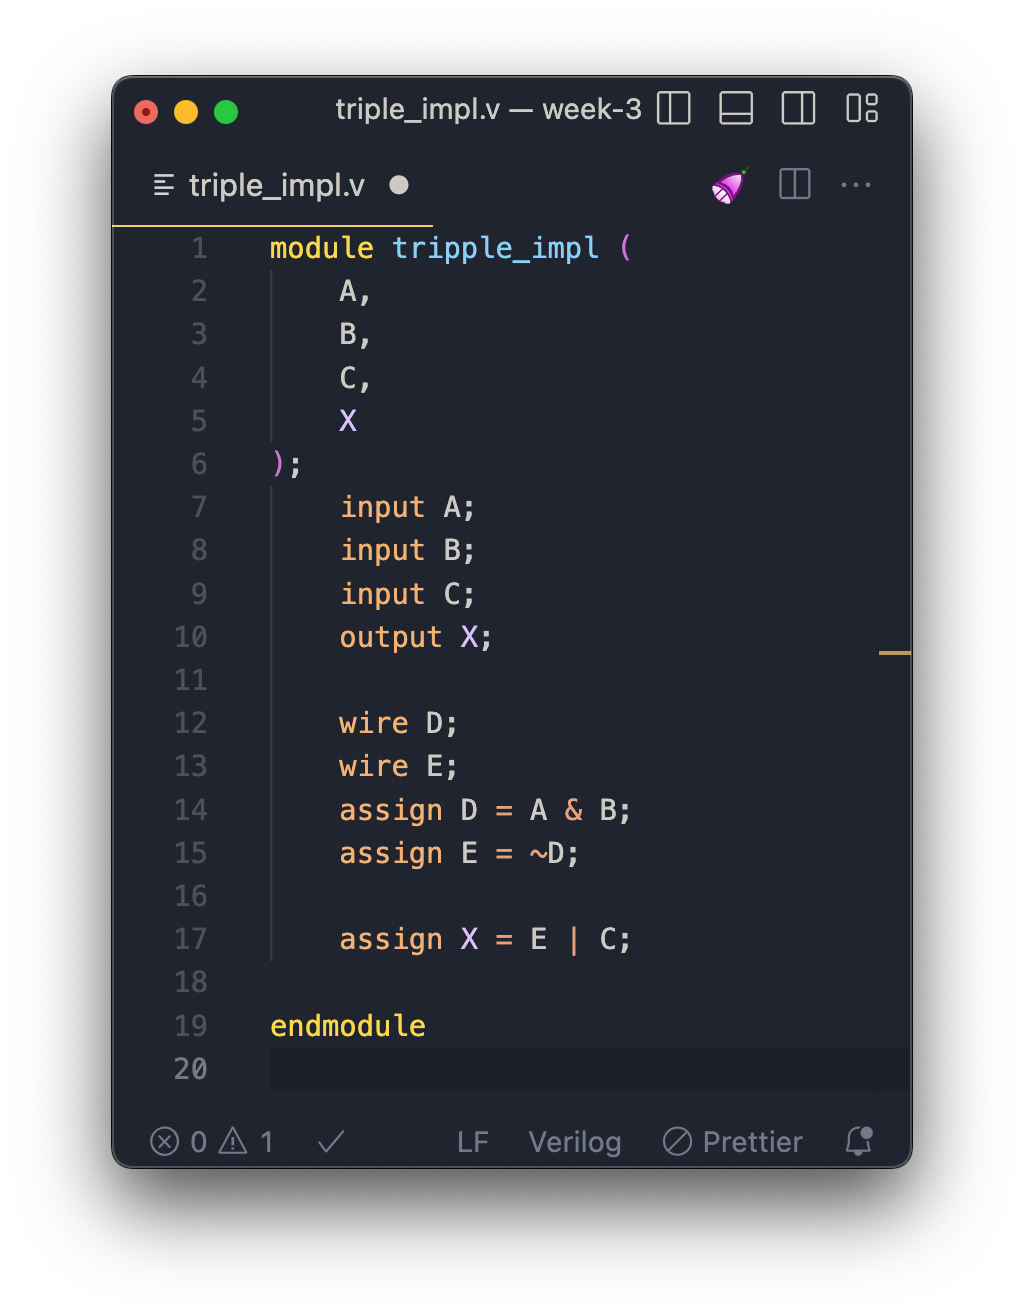
\includegraphics[width=10cm]{code-screenshot.png}
    \end{figure}
    
    \section*{Simulation \& Verification}

    here's the results of the simulation I ran.

    \begin{figure}[h]
        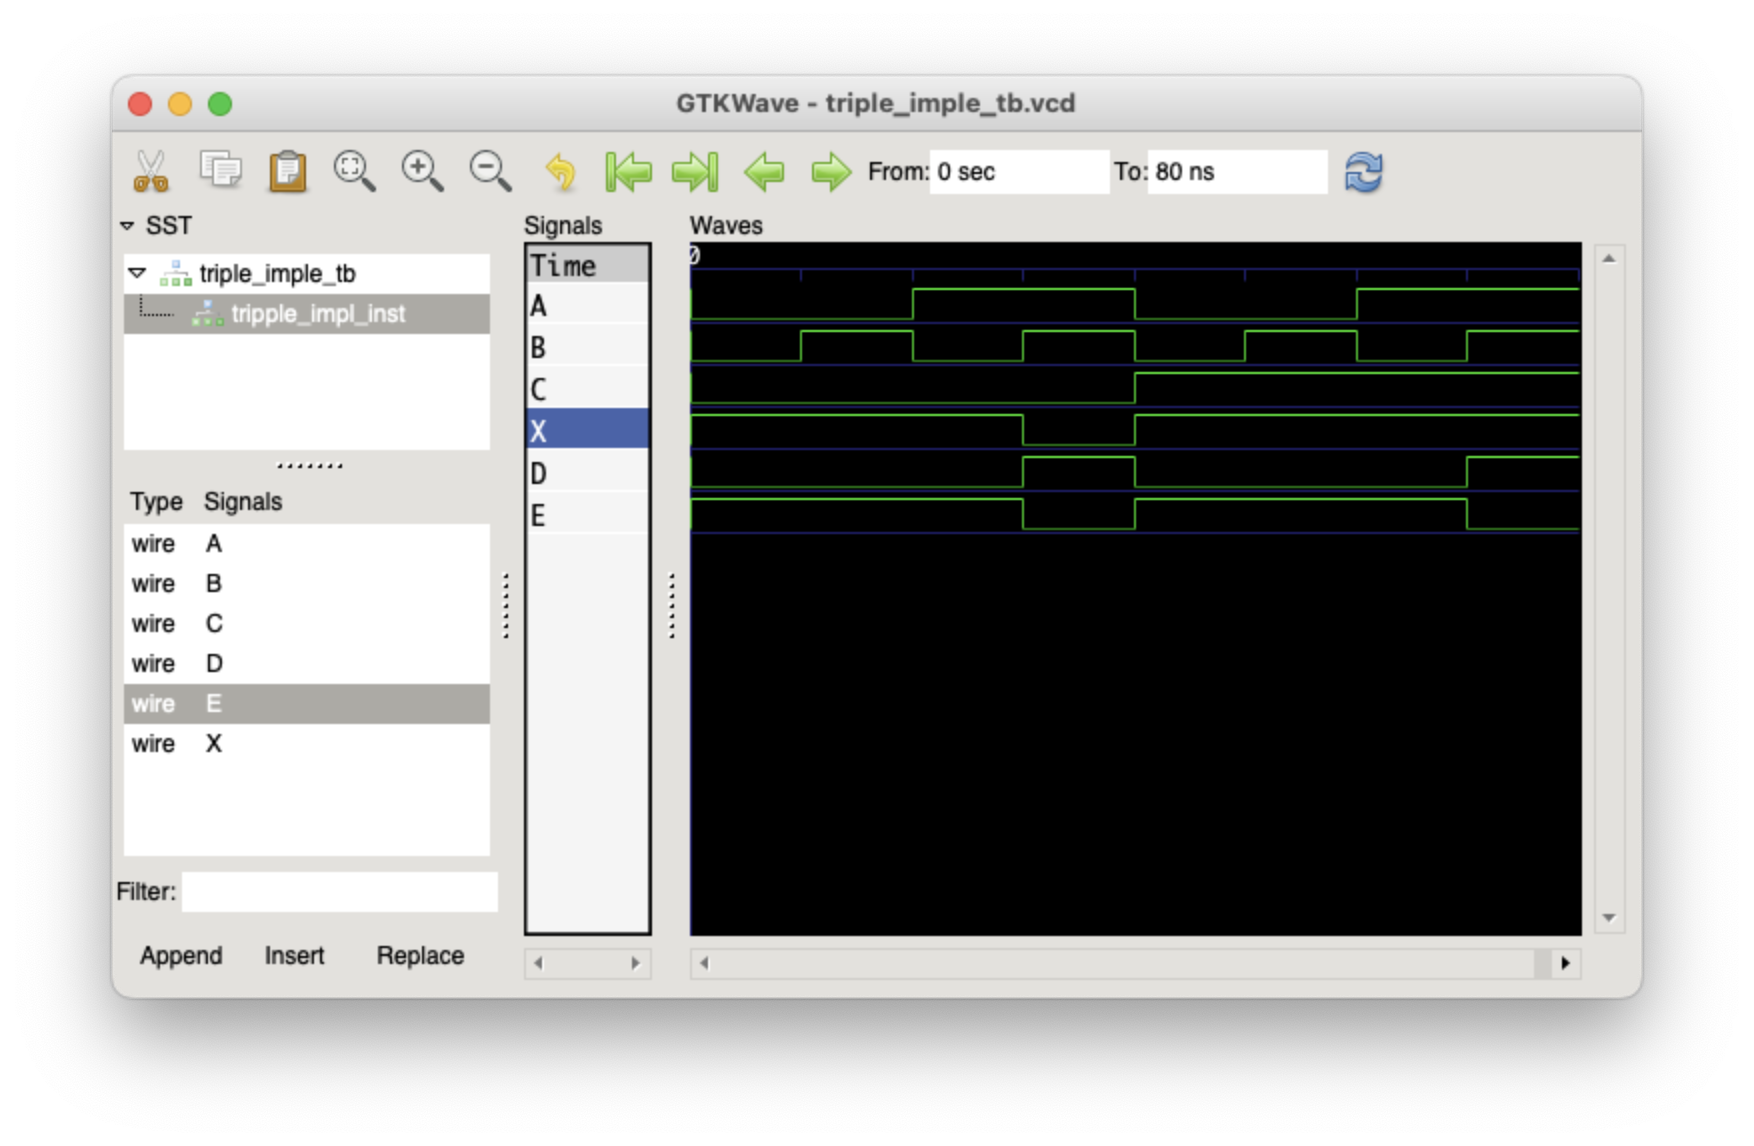
\includegraphics[width=12cm]{testing-screenshot.png}
    \end{figure}

    \section*{Conclusion}

    I had to do write verilog in VSCode, I hope it's written the way it was supposed to be.

    \section*{Reference}

    I used GTKWave for graphing the simulation results.

\end{document}